\documentclass[aspectratio=169,xcolor={usenames,dvipsnames},handout]{beamer}
% Handout Parameter, um die Foliensätze ohne einzelne "Klick-Schritte" zu generieren
%\documentclass[aspectratio=169,xcolor={usenames,dvipsnames}, handout]{beamer}
\usepackage[utf8x]{inputenc}
\usepackage[T1]{fontenc}
\usepackage{lmodern}
\usepackage[ngerman]{babel}
\usepackage{multimedia}
\usepackage{longtable}
\usepackage{array}
\usepackage{tikz}
\usepackage{listings}
\usepackage{caption}
\usepackage{transparent}
 
\usetheme{Szeged}

\beamertemplatenavigationsymbolsempty

\title{Kanban - ein Beispiel}
\author{Marcel Kaufmann}
\institute{PM QM - Hochschule Hannover}


\useoutertheme[footline=institutetitle]{miniframes}
\setbeamercolor{separation line}{use=structure,bg=structure.fg!50!bg}
\DeclareCaptionFont{white}{\color{white}}
\DeclareCaptionFormat{listing}{\colorbox{gray}{\parbox{\textwidth}{#1#2#3}}}
\captionsetup[lstlisting]{format=listing,labelfont=white,textfont=white}

\begin{document}

% Angepasster Footer mit Seitenzahlen (aktuell und max)
\setbeamertemplate{footline}
{
  \begin{beamercolorbox}[colsep=1.5pt]{upper separation line foot}
  \end{beamercolorbox}
\hbox{
\begin{beamercolorbox}[wd=0.5\paperwidth, ht=2.5ex, dp=1.125ex, left]{title in head/foot}
      \usebeamerfont{title in head/foot}\insertshorttitle
    \end{beamercolorbox}
\raggedright
\begin{beamercolorbox}[wd=0.5\paperwidth, ht=2.5ex, dp=1.125ex, right]{title in head/foot}
      \usebeamerfont{title in head/foot}\insertframenumber/\inserttotalframenumber\hspace*{2ex}
\end{beamercolorbox}
}
 \begin{beamercolorbox}[colsep=1.5pt]{lower separation line foot}
  \end{beamercolorbox}
}

% Strukturfarbe
\definecolor{flocksserver}{RGB}{0,100,0}

\setbeamercolor{normal text}{fg=black,bg=white}
\setbeamercolor{alerted text}{fg=red}
\setbeamercolor{example text}{fg=green!50!black}

\setbeamercolor{structure}{fg=flocksserver}
%\setbeamercolor{structure}{fg=Bittersweet}

\setbeamercolor{background canvas}{parent=normal text}
\setbeamercolor{background}{parent=background canvas}

\setbeamercolor{palette primary}{fg=yellow,bg=yellow} % changed this
\setbeamercolor{palette secondary}{use=structure,fg=structure.fg!100!green} % changed this
\setbeamercolor{palette tertiary}{use=structure,fg=structure.fg!100!green} % changed this


\begin{frame}
\titlepage
\end{frame}
\section{Kanban - ein Beispiel}

\subsection*{Kanban - ein Beispiel}

\begin{frame}
	\frametitle{Inhalt des Vortrags?}
		\begin{figure}[ht]
			
\includegraphics[width=6.5cm]{Bilder/fragerunde.png}
		\end{figure}
\end{frame}

\begin{frame}
	\frametitle{Unser Ziel}
	\begin{exampleblock}{Ziel}
		Unterschiede der Verfahren \emph{Push} und \emph{Pull} erleben, Metriken anwenden und vergleichen.
	\end{exampleblock}
\end{frame}

\begin{frame}
	\frametitle{Unsere Produktion}
	\begin{exampleblock}{Papierflieger bauen}
		Lean Production: Papierflieger bauen im Push- und Pull-Verfahren.
	\end{exampleblock}
	\begin{itemize}[<+->]
		\item 1 Manager/Projektleiter
		\item 1 Logistiker
		\item 4 Projektmitarbeiter
		\item (x) Beobachter
	\end{itemize}
\end{frame}
\begin{frame}
	\frametitle{Gruppen}
	\begin{exampleblock}{Eure Aufgabe}
		Gruppe bilden 6 + Beobachter
	\end{exampleblock}
	\pause
	\begin{itemize}[<+->]
			\item Rollen verteilen
			\item Projektmitarbeiter auf eine Seite (immer 1 Platz frei)
			\item Alle anderen stellen sich auf die andere Seite
		\end{itemize}
\end{frame}
\begin{frame}
	\frametitle{Eure Aufgabe Push-Vorgehen}
	\begin{exampleblock}{Aufgabe}
		Das folgende Szenario wird \textbf{5 Minuten} durchgespielt.
	\end{exampleblock}
	\begin{itemize}[<+->]
		\item Vier Prozessschritte für 4 Projektmitarbeiter
		\item Jeder Prozessschritt hat Ein- und Ausgang
		\item Prozess\textbf{kette} -> FIFO
		\item Logistiker transportiert Ware zwischen Ein- und Ausgang
		\item Manager/Projektleiter steuert verbal den Logistiker und achten auf Zeiten
		\item Manager/Projektleiter fügt in Minute 0:30 und 3:30 ein farbiges Papier ein um Durchlaufzeit zu messen (Zeit stoppen!)
		\item Beobachter beobachten den Verlauf und notieren Auffälligkeiten
		\item  Manager/Projektleiter und Beobachter füllen Metrikliste aus
	\end{itemize}
\end{frame}
\begin{frame}
	\begin{figure}[ht]
		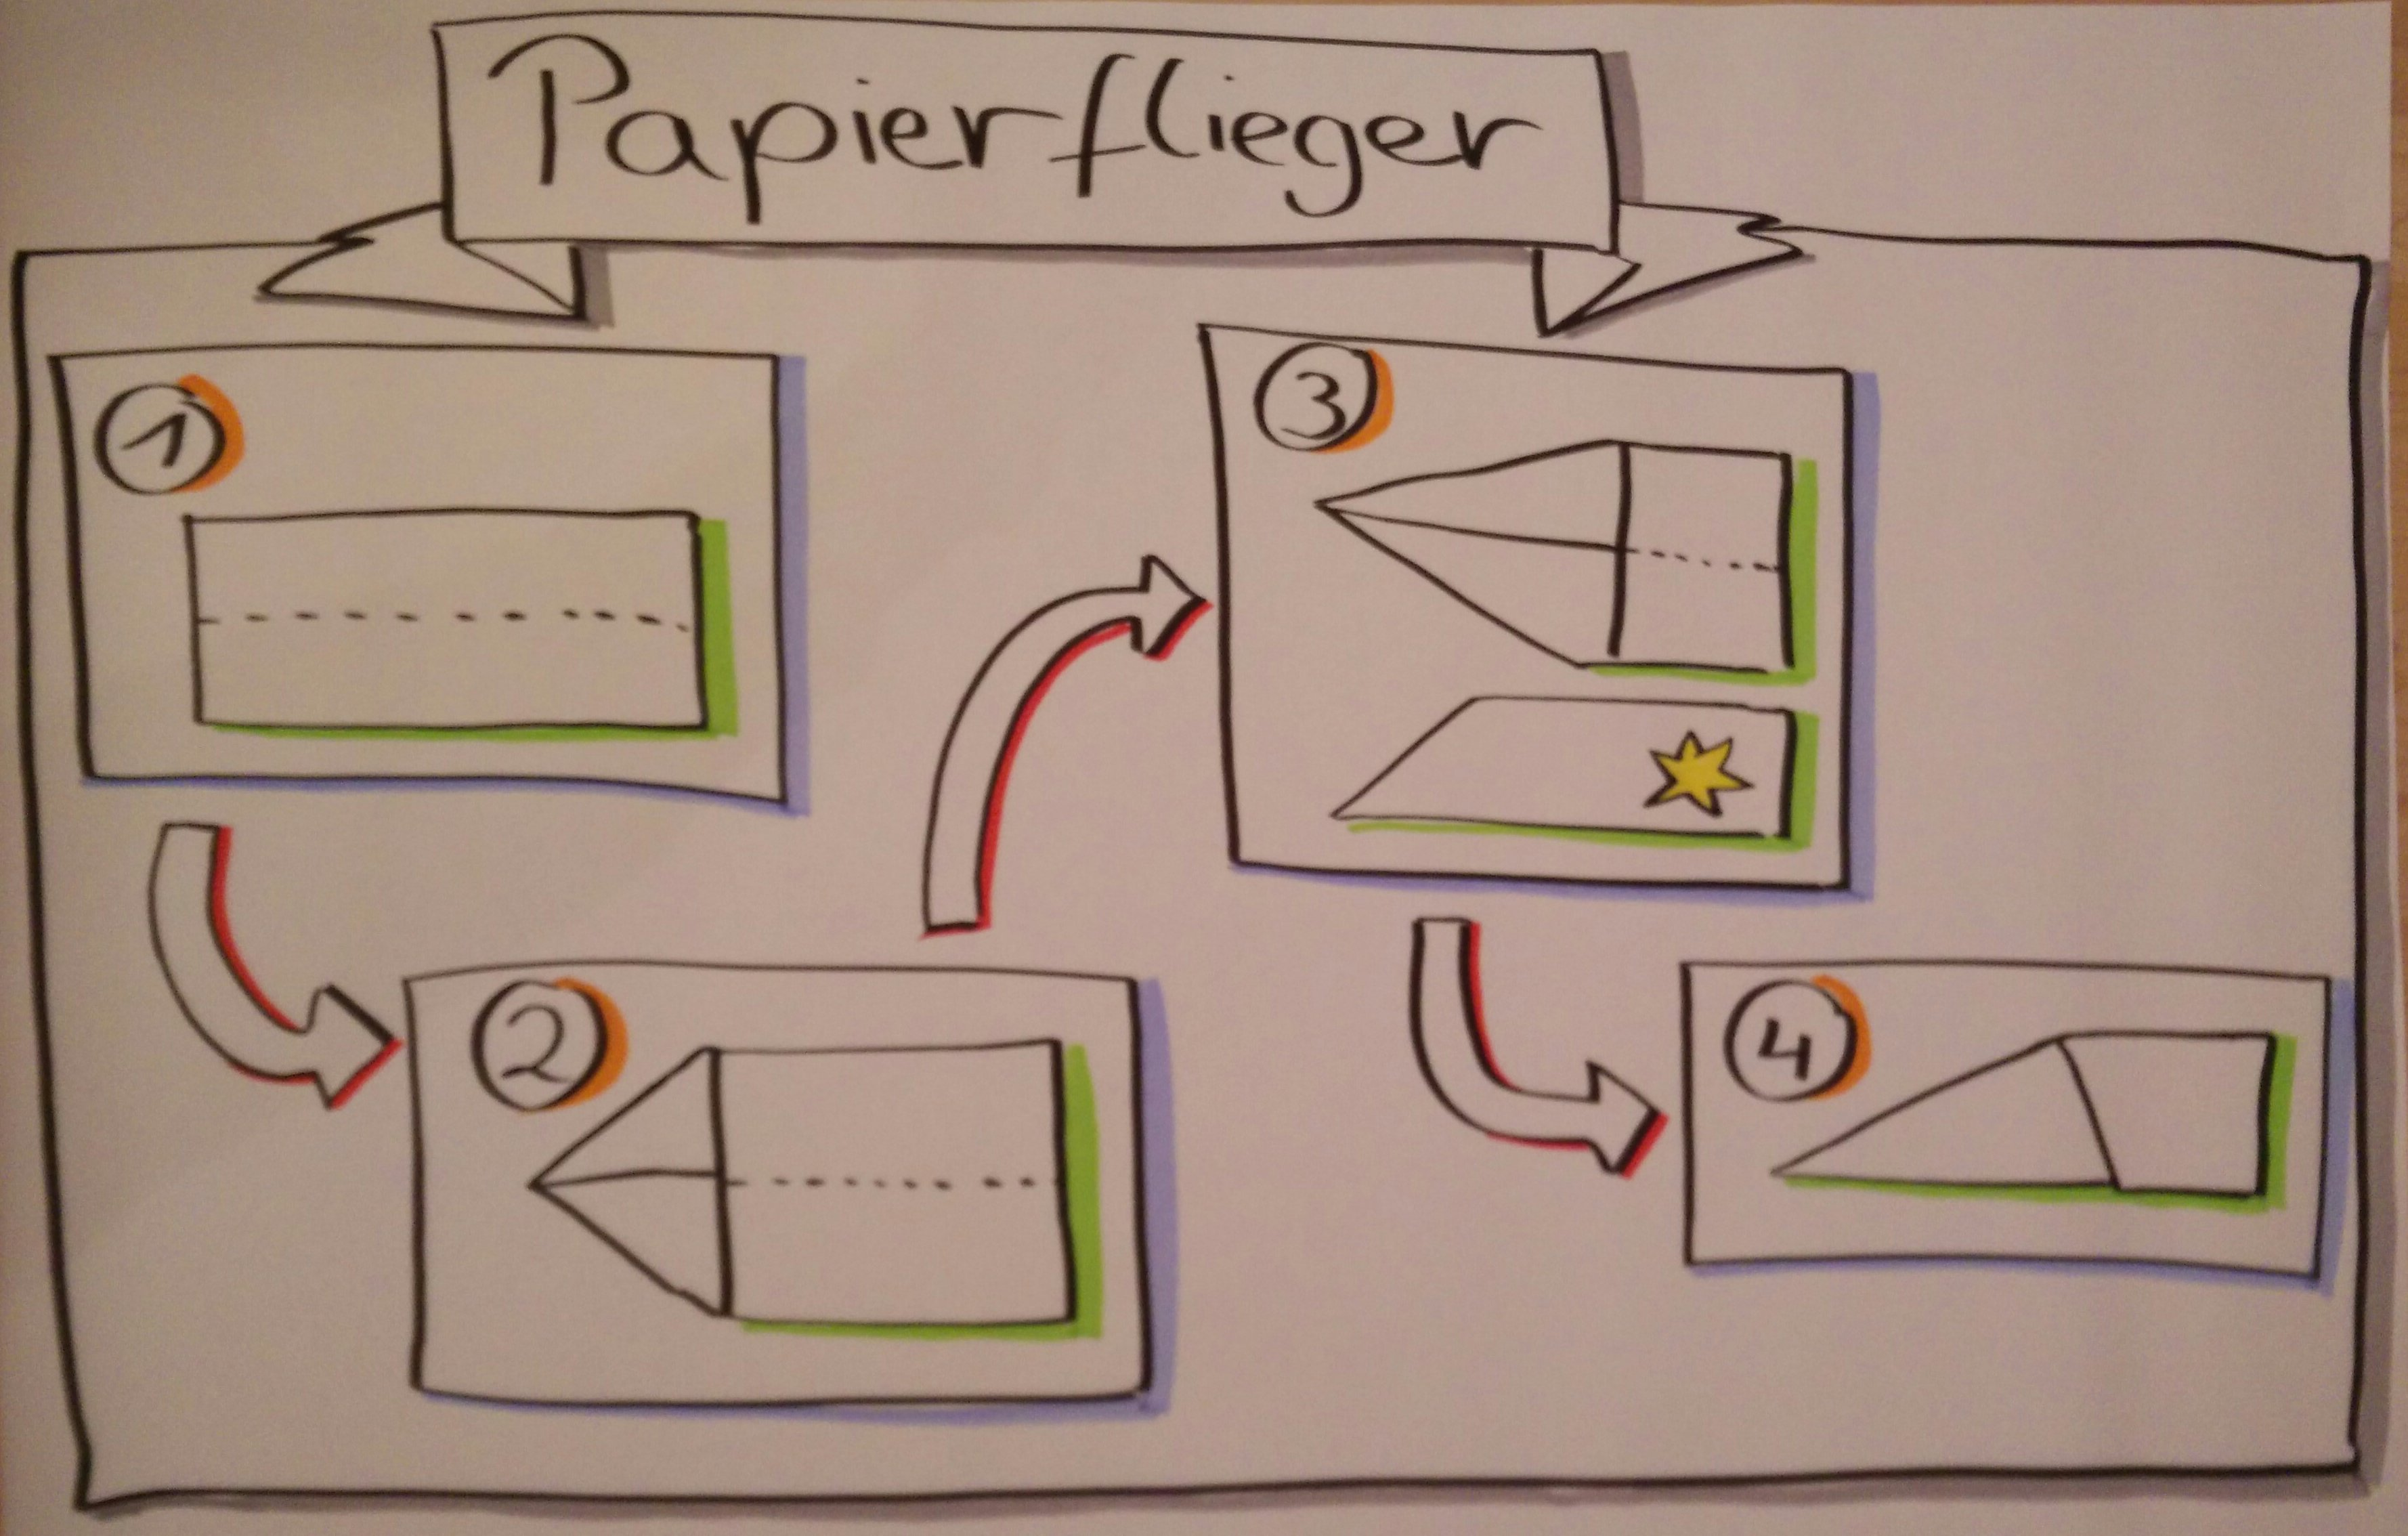
\includegraphics[width=10.9cm]{Bilder/papierflieger.jpg}
	\end{figure}
\end{frame}
\begin{frame}
	\frametitle{Eure Aufgabe Pull-Vorgehen}
	\begin{exampleblock}{Aufgabe}
		Das folgende Szenario wird \textbf{5 Minuten} durchgespielt.
	\end{exampleblock}
	\begin{itemize}[<+->]
		\item Vier Prozessschritte für 4 Projektmitarbeiter
		\item Jeder Prozessschritt hat \textbf{kombinierten} Ein- und Ausgang
		\item Kombinierte Ein- und Ausgänge dienen als Übergabepunkte
		\item Projektmitarbeiter nimmt nur \emph{neues} Material, wenn sein \emph{Ausgang} leer ist
		\item Manager fügt in Minute 0:30 und 3:30 ein farbiges Papier ein um Durchlaufzeit zu messen
		\item  Manager/Projektleiter und Beobachter füllen Metrikliste aus
	\end{itemize}
\end{frame}

\begin{frame}
	\frametitle{Auswertung}
	\begin{exampleblock}{Metriken}
		Auswertung und Besprechung der Ergebnisse einer Gruppe
	\end{exampleblock}
\end{frame}
\begin{frame}
	\frametitle{Fazit Push-Vorgehen}
	\begin{itemize}[<+->]
		\item Viele unfertige Produkte
		\item Lange Durchlaufzeiten
		\item Bei laufender Änderung hoher Ausschuss
		\item Spätes Erkennen von Fehlern teuer
		\item Hoher Aufwand für Logistik und Management
	\end{itemize}
\end{frame}
\begin{frame}
	\frametitle{Fragen und Antworten}
	\begin{figure}[ht]
		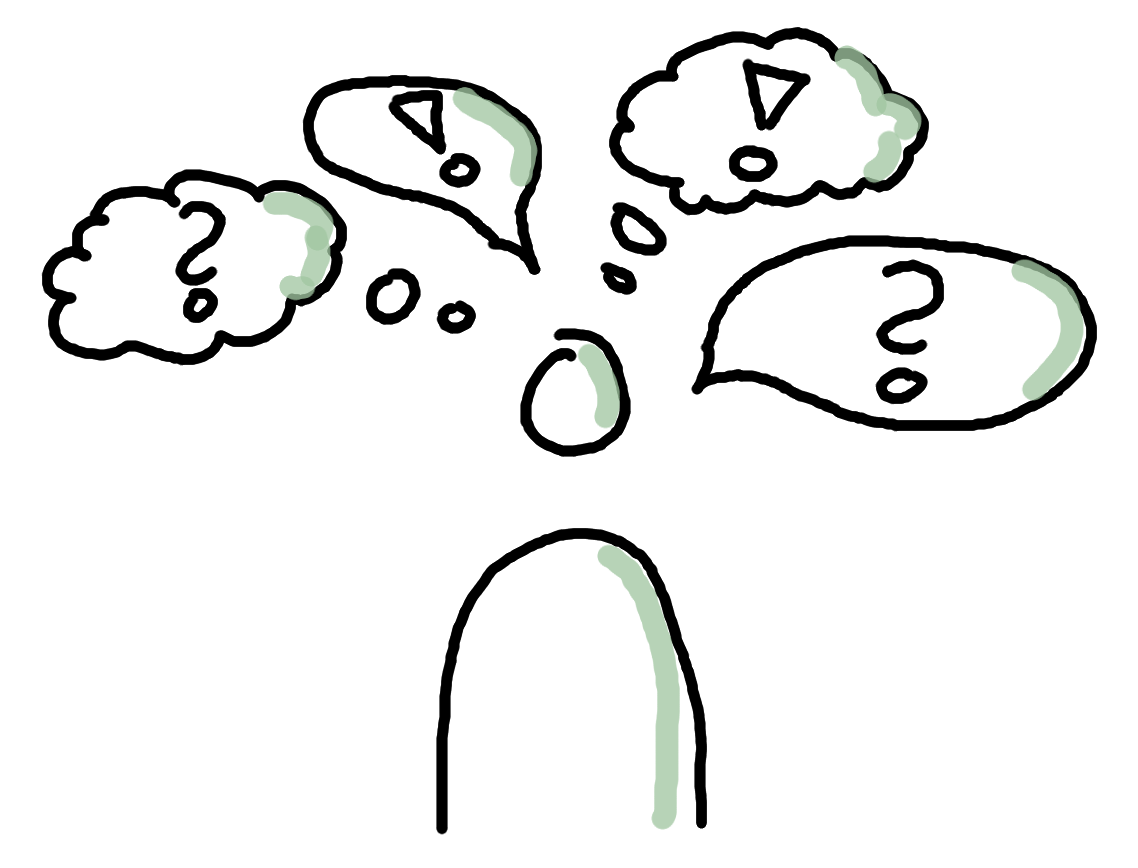
\includegraphics[width=8.0cm]{Bilder/fragenantwort.png}
	\end{figure}
\end{frame}
\begin{frame}[allowframebreaks]
	\frametitle{Quellen}
	\begin{thebibliography}{1}
		\bibitem{kanbanduell}
		Frank Besemer, Joachim Pfeffer, \emph{Das Kanban-Duell}, \url{http://www.scrum-day.de/files/scrum-day/content/upload/c4p-workshops-2014/Das\%20Kanban-Duell\%20-\%20Scrum\%20Day\%202014.pdf}, Aufruf: 30.11.2015 20:12 Uhr. \hskip 1em plus
		0.5em minus 0.4em
		
		\bibitem{wardenAirplane}
		Jesse Warden, \emph{Kanban Paper Airplane Factory}, \url{https://dzone.com/articles/kanban-paper-airplane-factory}, Aufruf: 30.11.2015 20:14 Uhr. \hskip 1em plus
		0.5em minus 0.4em
		
		\bibitem{leanorg}
		lean.org, \emph{Paper Airplane Activity}, \url{http://www.lean.org/FuseTalk/Forum/Attachments/Paper\%20Airplane\%20Activity.doc}, Aufruf: 30.11.2015 20:22 Uhr. \hskip 1em plus
		0.5em minus 0.4em
		
		\bibitem{simpleximprovement}
		simpleximprovement, \emph{Final Merged Simulation}, \url{https://www.youtube.com/watch?v=9exz80dGkfU}, Aufruf: 30.11.2015 20:37 Uhr. \hskip 1em plus
		0.5em minus 0.4em
		
		\bibitem{jitflow}
		leanaust.com, \emph{JIT Flow Simulation}, \url{http://leanaust.com/wp-content/uploads/2013/04/JIT-Flow-Simulation-Paper-Airplane-Simulation-Messier-Dowty.pdf}, Aufruf: 30.11.2015 20:55 Uhr. \hskip 1em plus
		0.5em minus 0.4em

	\end{thebibliography}
\end{frame}



\end{document}